El instrumental utilizado en las mediciones fue:
\begin{itemize}
\item Analizador vectorial de redes Agilent N9923A.
\item Analizador de espectros LPT-6000.
\item Generador de RF Agilent N9310A.
\end{itemize}

%%%%
\section{Analizador vectorial de redes}
%%%%

Al realizar una medición del coeficiente de reflexión del alimentador con el analizador vectorial de redes, existen 3 tipos de errores sistemáticos que se producen \cite{Agilent_vna_cal}:

\begin{itemize}
\item $\text{E}_{\text{D}}$ = Error por directividad.
\item $\text{E}_{\text{T}}$ = Error por seguimiento en reflexión.
\item $\text{E}_{\text{M}}$ = Error por desadaptación en la fuente.
\end{itemize}
En la figura \ref{fig_apE:1} se muestra un diagrama de flujo de la medición del coeficiente de reflexión $\Gamma$ en el que se incluyen los errores sistemáticos.
%%%%
\begin{figure} [H]
\centering 
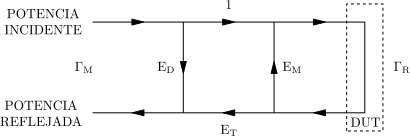
\includegraphics[scale = 1]{Figures/Apendice_E/ApendiceE_1.pdf}
\caption{Diagrama de flujo de la medición del coeficiente de reflexión $\Gamma$ con los errores sistemáticos incluidos.}
\label{fig_apE:1}
\end{figure}
%%%%
donde:
%%%%
\begin{align*}
\Gamma_{\text{M}} &= \text{Coeficiente de reflexión medido.}\\
\Gamma_{\text{R}} &= \text{Coeficiente de reflexión a determinar.}
\end{align*}
%%%%
A partir de la figura \ref{fig_apE:1}, se obtiene la expresión:
%%%%
\begin{align}
&\Gamma_{\text{M}} = \dfrac{\text{E}_{\text{D}} - \left(\text{E}_{\text{D}}\text{E}_{\text{M}} - \text{E}_{\text{T}}\right)\Gamma_{\text{R}}}{1 - \text{E}_{\text{M}}\Gamma_{\text{R}}}
\label{ec_apE:1}
\end{align}
%%%%
Para corregir los errores sistemáticos, es necesario realizar la calibración del analizador vectorial de redes, proceso que consiste en la medición del $\Gamma$ en tres condiciones de carga: cortocircuito, circuito abierto y una carga de 50 $\Omega$. De esta forma, se obtiene un sistema de 3 ecuaciones con 3 incógnitas a partir de las cuales pueden determinarse los errores sistemáticos, pudiendo así corregir la medición realizada.

A pesar de haber realizado correctamente la calibración del analizador vectorial de redes, no es posible eliminar completamente los errores sistemáticos producidos en la medición. Los errores remanantes luego de realizada la calibración se denominan \emph{errores residuales}, y son:
\begin{itemize}
\item $\delta$ = Error residual por directividad.
\item $\tau$ = Error residual por seguimiento en reflexión.
\item $\mu$ = Error residual por desadaptación en la fuente.
\end{itemize}
Las incertezas producidas en la medición del módulo y de la fase del $\Gamma$ dependen de los errores residuales, y pueden expresarse como \cite{Agilent_vna_err}:
%%%%
\begin{subequations}
\label{grup_ec_apE:1}
\begin{align}
\Delta\left|\Gamma\right| &= \delta + \left(1 - \tau\right)\left|\Gamma\right| +  \mu\left|\Gamma\right|^2 + \left(1 - \text{A}\right)\left|\Gamma\right|
\label{ec_apE:2}\\
\Delta\angle\Gamma &= \arcsen\left(\dfrac{\Delta\left|\Gamma\right|}{\Gamma}\right)
\label{ec_apE:3}
\end{align}
\end{subequations}
%%%%
donde:
\begin{align*}
&\text{A} = \text{Error por precisión dinámica.}
\end{align*}
%%%%
Los errores se determinan a partir de las especificaciones del instrumento de medición; dado que los errores se encuentran especificados en dB, es necesario convertirlos a valores lineales antes de calcular las incertezas. Para el analizador vectorial de redes utilizado, las especificaciones \cite{Agilent_vna_man} y las conversiones a valores lineales se muestran en la tabla \ref{tabla_apE:1}.
%%%%
\begin{table}[H]
\centering
\begin{tabular}{|c|c|c|}
\hline
Error & Especificación (dB) & Valor lineal\\
\hline
$\delta$ & 42 & 0,008\\
\hline
$\tau$ & $\pm$0,06 & 0,993\\
\hline
$\mu$ & 36 & 0,016\\
\hline
A & 0,1 & 0,989\\
\hline
\end{tabular}
\caption{Especificaciones de los errores del analizador vectorial de redes Agilent N9923A y sus conversiones a valores lineales.}
\label{tabla_apE:1}
\end{table}
%%%%
En la medición del alimentador realizada con el analizador vectorial de redes, los valores de magnitud y fase obtenidos son:
%%%%
\begin{align*}
\left|\Gamma\right| &= \text{0,03027143427466} \simeq \text{0,030}\\
\angle\Gamma &= \text{0,05388041135260 rad} \simeq \text{0,054 rad}
\end{align*}
%%%%
Empleando las expresiones \eqref{grup_ec_apE:1}, las incertezas producidas en la medición del módulo y de la fase del $\Gamma$ del alimentador son:
%%%%
\begin{align*}
\left|\Delta\left|\Gamma\right|\right| &= \text{0,00851270700079} \simeq \text{0,009}\\
\left|\Delta\angle\Gamma\right| &= \text{0,28505740750033 rad} \simeq \text{0,285 rad}
\end{align*}
%%%%
A partir de la expresión de la relación de onda estacionaria:
%%%%
\begin{align}
&\text{ROE} = \dfrac{1 + \left|\Gamma\right|}{1 - \left|\Gamma\right|}
\label{ec_apE:4}
\end{align}
%%%%
y aplicando propagación de errores \cite{walfram_error_prop}, se determina la incerteza producida en la medición de la ROE como:
%%%%
\begin{align}
&\left|\Delta\text{ROE}\right| = \dfrac{2}{\left(1 - \left|\Gamma\right|\right)^2}\left|\Delta\left|\Gamma\right|\right|
\label{ec_apE:5}
\end{align}
%%%%
Empleando la expresión \eqref{ec_apE:5}, la incerteza producida en la medición de la ROE es:
%%%%
\begin{align*}
&\left|\Delta\text{ROE}\right| = \text{0,01810494889657} \simeq \text{0,02}
\end{align*}
%%%%
Las partes real e imaginaria del $\Gamma$ del alimentador se determinan a partir del módulo y de la fase a partir de las expresiones:
%%%%
\begin{subequations}
\label{grup_ec_apE:2}
\begin{align}
\Re\!\left(\Gamma\right) &= \left|\Gamma\right|\cos\left(\angle\Gamma\right)
\label{ec_apE:6}\\
\Im\!\left(\Gamma\right) &= \left|\Gamma\right|\sen\left(\angle\Gamma\right)
\label{ec_apE:7}
\end{align}
\end{subequations}
%%%%
A partir de las expresiones \eqref{grup_ec_apE:2} y aplicando propagación de errores, se determinan las incertezas producidas en las partes real e imaginaria del $\Gamma$ del alimentador como:
%%%%
\begin{subequations}
\label{grup_ec_apE:3}
\begin{align}
\left|\Delta\Re\!\left(\Gamma\right)\right| &= \left|\cos\left(\angle\Gamma\right)\right|\left|\Delta\left|\Gamma\right|\right| + \left|\Gamma\right|\left|\sen\left(\angle\Gamma\right)\right|\left|\Delta\angle\Gamma\right|
\label{ec_apE:8}\\
\left|\Delta\Im\!\left(\Gamma\right)\right| &= \left|\sen\left(\angle\Gamma\right)\right|\left|\Delta\left|\Gamma\right|\right| + \left|\Gamma\right|\left|\cos\left(\angle\Gamma\right)\right|\left|\Delta\angle\Gamma\right|
\label{ec_apE:9}
\end{align}
\end{subequations}
%%%%
Empleando las expresiones \eqref{grup_ec_apE:3}, las incertezas producidas en las partes real e imaginaria del $\Gamma$ del alimentador son:
%%%%
\begin{align*}
\left|\Delta\Re\!\left(\Gamma\right)\right| &= \text{0,00896506772042} \simeq \text{0,009}\\
\left|\Delta\Im\!\left(\Gamma\right)\right| &= \text{0,00907502030661} \simeq \text{0,009}
\end{align*}
%%%%
Las partes real e imaginaria de la impedancia del alimentador $Z_L$ se determinan a partir del módulo y de la fase del $\Gamma$:
%%%%
\begin{subequations}
\label{grup_ec_apE:4}
\begin{align}
\Re\!\left(Z_L\right) &= Z_O\dfrac{1 - \Re\!\left(\Gamma\right)^2 - \Im\!\left(\Gamma\right)^2}{\left[1 - \Re\!\left(\Gamma\right)\right]^2 + \Im\!\left(\Gamma\right)^2}
\label{ec_apE:10}\\
\Im\!\left(Z_L\right) &= Z_O\dfrac{2\Im\!\left(\Gamma\right)}{\left[1 - \Re\!\left(\Gamma\right)\right]^2 + \Im\!\left(\Gamma\right)^2}
\label{ec_apE:11}
\end{align}
\end{subequations}
%%%%
A partir de las expresiones \eqref{grup_ec_apE:4} y aplicando propagación de errores, se determinan las incertezas producidas en las partes real e imaginaria de la impedancia del alimentador como:
%%%%
\begin{subequations}
\label{grup_ec_apE:5}
\begin{align}
\left|\Delta\Re\!\left(Z_L\right)\right| &= \left|\dfrac{2Z_0\left\{\!\left[1 - \Re\!\left(\Gamma\right)\right]^2 - \Im\!\left(\Gamma\right)^2\right\}}{\left\{\!\left[1 - \Re\!\left(\Gamma\right)\right]^2 + \Im\!\left(\Gamma\right)^2\right\}^2}\right|\left|\Delta\Re\!\left(\Gamma\right)\right| + \left|\dfrac{4Z_0\left[1 - \Re\!\left(\Gamma\right)\right]\Im\!\left(\Gamma\right)}{\left\{\!\left[1 - \Re\!\left(\Gamma\right)\right]^2 + \Im\!\left(\Gamma\right)^2\right\}^2}\right|\left|\Delta\Im\!\left(\Gamma\right)\right|
\label{ec_apE:12}\\
\left|\Delta\Im\!\left(Z_L\right)\right| &= \left|\dfrac{4Z_0\left[1 - \Re\!\left(\Gamma\right)\right]\Im\!\left(\Gamma\right)}{\left\{\!\left[1 - \Re\!\left(\Gamma\right)\right]^2 + \Im\!\left(\Gamma\right)^2\right\}^2}\right|\left|\Delta\Re\!\left(\Gamma\right)\right| + \left|\dfrac{2Z_0\left\{\!\left[1 - \Re\!\left(\Gamma\right)\right]^2 - \Im\!\left(\Gamma\right)^2\right\}}{\left\{\!\left[1 - \Re\!\left(\Gamma\right)\right]^2 + \Im\!\left(\Gamma\right)^2\right\}^2}\right|\left|\Delta\Im\!\left(\Gamma\right)\right|
\label{ec_apE:13}
\end{align}
\end{subequations}
%%%%
Empleando las expresiones \eqref{grup_ec_apE:5}, las incertezas producidas en la medición de las partes real e imaginaria de la impedancia del alimentador son:
%%%%
%%%%
\begin{align*}
\left|\Delta\Re\!\left(Z_L\right)\right| &= \text{0,84740126818922 }\Omega \simeq \text{0,85 }\Omega\\
\left|\Delta\Im\!\left(Z_L\right)\right| &= \text{0,85772757113368 }\Omega \simeq \text{0,86 }\Omega
\end{align*}
%%%%

%%%%
\section{Analizador de espectros}
%%%%

Las incertezas producidas al realizar una medición de amplitud con el analizador de espectros \cite{Agilent_an_esp_err} se determinan a partir de sus especificaciones. Para el analizador de espectros utilizado, las especificaciones son \cite{LPT_ana_esp_man}:
\begin{itemize}
\item Error por respuesta en frecuencia = $\pm$1,5 dB.
\item Error por fidelidad de la escala de la pantalla = $\pm$1,5 dB (10 dB/div).
\end{itemize}
La incerteza total producida en mediciones de amplitud es:
%%%%
\begin{align*}
\left|\Delta\text{A}\right| &= 3 \text{ dB}
\end{align*}
%%%%
La incerteza producida en la medición del ancho de haz (\ref{subsec_intro_diag_rad}) depende solamente de la incerteza en el ángulo $\uptheta$:
%%%%
\begin{align*}
\left|\Delta\uptheta\right| &= \text{1,5}^{\circ}
\end{align*}
%%%%
La incerteza resultante en la medición del ancho de haz se expresa como:
%%%%
\begin{align*}
\left|\Delta\text{Ancho de haz}\right| &= 2\left|\Delta\uptheta\right| = 3^{\circ}
\end{align*}
%%%%
Para la medición de $G_{fn}\left(\theta_0\right)$ (\ref{subsec_principios_efi_glo_ilu}), se toma el valor más cercano a  $\theta_0$. Considerando que  $\theta_0 = 71,5^{\circ}$, en la tabla \ref{tabla_apE:2} se muestran las cotas de error resultantes.
%%%%
\begin{table}[H]
\centering
\begin{tabular}{|c|c|c|c|c|}
\hline
\multirow{2}{*}{Plano} & Cota inferior & Ganancia en cota & Cota superior & Ganancia en cota\\
& (grados) & inferior (dB) & (grados) & superior (dB)\\
\hline
E & 70,17 & -7,01 & 71,69 & -7,33\\
\hline
H & 70,53 & -8,60 & 72,00 & -8,91\\
\hline
\end{tabular}
\caption{Cotas de error en la medición de $G_{fn}\left(\theta_0\right)$.}
\label{tabla_apE:2}
\end{table}
%%%%
Tomando los ángulos más cercanos a $\theta_0$, las mediciones de $G_{fn}\left(\theta_0\right)$ son:
\begin{align*}
G_{fn}\left(\theta_0\right) &= -\text{7,33 dB (Plano E)}\\
G_{fn}\left(\theta_0\right) &= -\text{8,91 dB (Plano H)}
\end{align*}
%%%%
La incerteza en la medición de $G_{fn}\left(\theta_0\right)$ depende de las incertezas $\left|\Delta\text{A}\right|$ y $\left|\Delta\uptheta\right|$. Considerando que en los planos E y H la diferencia en la ganancia es de aproximadamente 0,3 dB, la incerteza de $G_{fn}\left(\theta_0\right)$ queda expresada como:
%%%%
\begin{align*}
\left|\Delta G_{fn}\left(\theta_0\right)\right| &= \left|\Delta\text{A}\right| + \dfrac{0,3 \text{ dB}}{2} = 3,15 \text{ dB}
\end{align*}
%%%%
La incerteza en la medición de la relación frente-espalda se expresa como:
%%%%
\begin{align*}
\left|\Delta\text{Relación frente-espalda}\right| &= 2\left|\Delta\text{A}\right| = 6 \text{ dB}
\end{align*}
%%%%